\section{OSRKit}

In this section we present a preliminar experimental study of \osrkit. In particular, we aim at addressing the following questions:

\begin{description}[labelindent=1em ,labelsep*=1em,leftmargin=3.5em,itemsep=3pt,parsep=3pt]
\item[Q1] How much does a never-firing OSR point impact code quality? What kind of slowdown should we expect?
\item[Q2] What is the run-time overhead of an OSR transition, for instance to a clone of the running function?
\item[Q3] What is the overhead of \osrkit\ for inserting OSR points and creating a stub or a continuation function?
\end{description}

\missing


\subsection{Experimental Setup}

\subsubsection*{Benchmarks}
We address questions Q1-Q3 by analyzing the performance of \osrkit\ on a selection of the \shootout\ benchmarks, also known as the Computer Language Benchmarks Game~\cite{shootout}, running in \tinyvm. In particular, we focus on single-threaded benchmarks that do not rely on external libraries to perform their core computations. Benchmarks and their description are reported in \mytable\ref{tab:osr-shootout}; four of them ({\tt b-trees}, {\tt mbrot}, {\tt n-body} and {\tt sp-norm}) are evaluated against two workloads of different size.

\begin{table}[ht]
\begin{center}
\begin{small}
    \begin{tabular}{ |c|c| }
        \hline
        Benchmark & Description \\
        \hline
        \hline
        b-trees & Adaptation of a GC bench for binary trees \\
        \hline
        fannkuch & Fannkuch benchmark on permutations \\
        \hline
        fasta & Generation of DNA sequences \\
        \hline
        fasta-redux & Generation of DNA sequences (with lookup table) \\
        \hline
        mbrot & Mandelbrot set generation \\
        \hline
        n-body & N-body simulation of Jovian planets \\
        \hline
        rev-comp & Reverse-complement of DNA sequences \\
        \hline
        sp-norm & Eigenvalue calculation with power method \\
        \hline
    \end{tabular}
\end{small}
\end{center}
\caption{\label{tab:osr-shootout} Description of the \shootout\ benchmarks.}
\end{table}

We generate the IR modules for our experiments with \clang\ starting from the C version of the \shootout\ suite. To cover scenarios where OSR machinery is inserted in programs with different optimization levels, we consider two versions: 1) {\em unoptimized}, where the only LLVM optimization we perform is \memtoreg\ to promote stack references to registers and construct the SSA form; 2) {\em optimized}, where we apply {\tt opt} {\tt -O1} to the unoptimized version.

\subsubsection*{Environment}
\tinyvm\ supports interactive invocations of functions and it can compile LLVM IR either generated at run-time or loaded from disk. The main design goal behind \tinyvm\ is the creation of an interactive environment for IR manipulation and JIT-compilation of functions: for instance, it allows the user to insert OSR points in loaded functions, run optimization passes on them or display their CFGs, repeatedly invoke a function for a specified amount of times and so on.

\tinyvm\ supports dynamic library loading and linking, and comes with a helper component for MCJIT that simplifies tasks such as handling multiple IR modules, symbol resolution in the presence of multiple versions of a function, and tracking native code and other machine-level generated object such as Stackmaps. \tinyvm\ is thus an ideal playground to exercise our OSR technique.

\subsubsection*{Platform}
Experiments were performed on an octa-core 2.3Ghz Intel Xeon E5-4610 v2 with 256+256KB of L1 cache, 2MB of L2 cache, 16MB of shared L3 cache, and 128 GB of DDR3 main memory, running Debian Wheezy 7, Linux kernel 3.2.0, LLVM 3.6.2 (Release build, compiled using gcc 4.7.2), 64 bit. For each benchmark we analyze CPU time performing 10 trials preceded by an initial warm-up iteration; reported confidence intervals are stated at 95\% confidence level.

\subsection{Impact on Code Quality}

\ifdefined\noauthorea
\begin{figure}[!ht]
\begin{center}
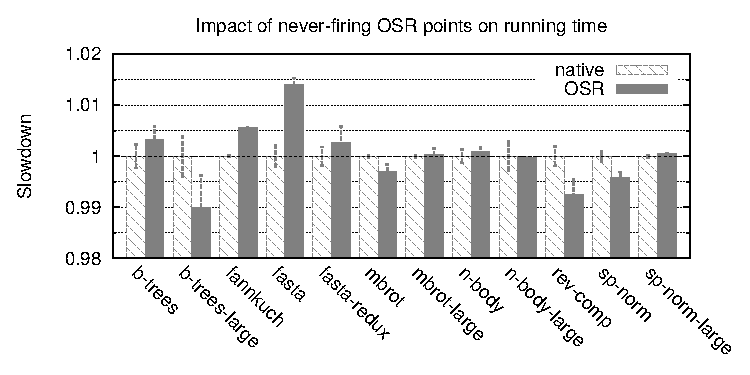
\includegraphics[width=0.65\textwidth]{figures/osr-code-quality-base/osr-code-quality-base.eps}
\caption{\protect\label{fig:osr-code-quality-base} Q1: Impact on running time of never-firing OSR points inserted inside hot code portions (unoptimized code).


}
\end{center}
\end{figure}
\fi

\ifdefined\noauthorea
\begin{figure}[ht]
\begin{center}
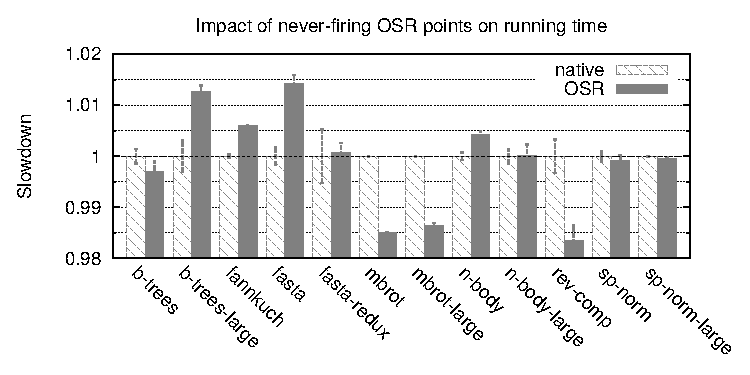
\includegraphics[width=0.65\textwidth]{figures/osr-code-quality-O1/osr-code-quality-O1.eps}
\caption{\protect\label{fig:osr-code-quality-O1} Q1: Impact on running time of never-firing OSR points inserted inside hot code portions (optimized code).



}
\end{center}
\end{figure}
\fi

In order to measure how much a never-firing OSR point might impact code quality (Q1), we analyzed the source-code structure of each benchmark and profiled its run-time behavior to identify performance-critical sections for OSR point insertion. The distinction between open and resolved OSR points is nearly irrelevant in this context: we choose to focus on open OSR points, passing {\tt null} as the {\tt val} argument for the stub (see \missing).

For iterative benchmarks, we insert an OSR point in the body of their hottest loops. We classify a loop as hottest when its body is executed for a very high cumulative number of iterations (e.g., from millions up to billions) and it either calls the method with the highest {\em self} time in the program, or it performs the most computational-intensive operations for the program in its own body.

These loops are natural candidates for OSR point insertion: for instance, the Jikes RVM inserts yield points on backward branches to trigger operations such as method recompilation through OSR and thread preemption for garbage collection. In the \shootout\ benchmarks, the number of such loops is typically 1 (2 for {\tt spectral-norm}).

For recursive benchmarks, we insert an OSR point in the body of the method that accounts for the largest {\em self} execution time in the program. Such an OSR point might be useful to trigger recompilation of the code at a higher degree of optimization, enabling for instance multiple levels of inlining for non-tail-recursive functions. The only analyzed benchmark showing a recursive pattern is {\tt b-trees}.

Results for the unoptimized and optimized versions of the benchmarks are reported in \myfigure\ref{fig:osr-code-quality-base} and \myfigure\ref{fig:osr-code-quality-O1}, respectively. For both scenarios we observe that the overhead is very small, i.e., less than $1\%$ for most benchmarks and less than $2\%$ in the worst case. For some benchmarks, code might run slightly faster after OSR point insertion due to instruction cache effects.
%We analyzed the code produced by the x86-64 back-end: the OSR machinery is lowered into three native instructions that load a counter in a register, compare it against a constant value and jump to the OSR block accordingly.
The number of times the OSR condition is checked for each benchmark is
%the same as in the experiments
reported in \mytable\ref{tab:osr-sameFun}.

\subsection{Overhead of OSR Transitions}

\mytable\ref{tab:osr-sameFun} reports estimates of the average cost of performing an OSR transition to a clone of the running function (Q2). For each benchmark we compute the time difference between the scenarios in which an always-firing and a never-firing resolved OSR point is inserted in the code, respectively; we then normalize this difference against the number of fired OSR transitions.

\begin{table}[ht]
\begin{center}
\begin{small}
    \begin{tabular}{ |c|C{1.33cm}|C{1.00cm}|C{1.15cm}|C{1.00cm}|C{1.15cm}| }
        \cline{3-6}
        \multicolumn{2}{c|}{} & \multicolumn{2}{c|}{{\em Unoptimized code}} & \multicolumn{2}{c|}{{\em Optimized code}} \\
        \hline
        Benchmark & Fired OSRs (M) & Live values & Avg time (ns) & Live values & Avg time (ns) \\
        \hline
        \hline
        b-trees & 605 & 2 & 1.731 & 3 & 0.974 \\
        \hline
        b-trees-large & 2\,690 & 2 & 1.749 & 3 & 1.423 \\
        \hline
        fannkuch & 399 & 0 & 1.793 & 0 & 0.621 \\
        \hline
        fasta & 400 & 2 & 2.335 & 2 & 2.699 \\
        \hline
        fasta-redux & 400 & 4 & 2.306 & 4 & 2.269 \\
        \hline
        mbrot & 256 & 15 & 5.016 & 15 & 3.628 \\
        \hline
        mbrot-large & 1\,024 & 15 & 5.268 & 15 & 4.637 \\
        \hline
        n-body & 50 & 3 & 2.952 & 3 & 6.929 \\
        \hline
        n-body-large & 500 & 3 & 2.953 & 3 & 6.953 \\
        \hline
        rev-comp & 6 & 8 & -10.158 & 8 & 8.267 \\
        \hline
        sp-norm & 1\,210 & 2 & 0.772 & 2 & -0.030 \\
        \hline
        sp-norm-large & 19\,360 & 2 & 0.778 & 2 & -0.003 \\
        \hline
    \end{tabular}
\end{small}
\end{center}
\caption{\label{tab:osr-sameFun}Cost of OSR transitions to the same function. For each benchmark we report the number of fired OSR transitions (rounded to millions), the number of live values passed at the OSR point, and the average time for a transition.
}
\end{table}

Hot code portions for OSR point insertion have been identified as in the Q1 experiments for code quality. Depending on the characteristics of the hot loop, we either transform its body into a separate function and instrument its entrypoint, or, when the loop calls a method with a high self time, we insert an OSR point at the beginning of that method.

Normalized differences reported in the table represent a reasonable estimate of the average cost of firing an OSR transition.
%, which in other words is the cost of performing a function call passing the live variables as arguments.
Reported numbers are in the order of nanoseconds, and might be negative due to instruction cache effects. We remark that for this experiment slicing the loop body is preferable to inserting an OSR point in it, as the continuation function should fire an OSR itself at the very next loop iteration and so on, possibly leading to an undesired stack growth.

\subsection{OSR Machinery Generation}

We now discuss the overhead of the \osrkit\ library for inserting OSR machinery in the IR of a function (Q3). \mytable\ref{tab:osr-instrTime} reports for each benchmark the number of IR instructions in the instrumented function and the time spent in the IR manipulation. Locations for OSR points are chosen as in the Q1 experiments, and the target function is a clone of the source function.

\begin{table}[ht]
\begin{small}
    \begin{tabular}{ |c|c|c|c|c|c|c| }
        \cline{3-7}
        \multicolumn{2}{l|}{} & \multicolumn{2}{c|}{{\em Open OSR {\tiny$(\mu s)$}}} & \multicolumn{3}{c|}{{\em Resolved OSR  {\tiny$(\mu s)$}}} \\
        \cline{3-7}
        \multicolumn{2}{l|}{} & Insert & Gen. & Insert & \multicolumn{2}{|c|}{Generate \fosrto} \\
        \cline{1-2} \cline{6-7}
        Benchmark & \textbar IR\textbar & point & stub & point & Total & Avg/inst \\
        \hline
        \hline
        b-trees & 13 & 15.40 & 28.32 & 14.31 & 76.13 & 5.86 \\
        \hline
        fannkuch & 50 & 14.16 & 18.66 & 12.84 & 208.03 & 4.16 \\
        \hline
        fasta & 38 & 12.93 & 27.07 & 13.01 & 250.39 & 6.59 \\
        \hline
        fasta-redux & 55 & 13.79 & 23.44 & 9.32 & 258.36 & 4.70 \\
        \hline
        mbrot & 77 & 15.96 & 27.39 & 15.30 & 384.61 & 4.99 \\
        \hline
        n-body & 19 & 14.31 & 19.73 & 11.58 & 88.73 & 4.67  \\
        \hline
        rev-comp & 145 & 16.31 & 39.99 & 13.90 & 810.84 & 5.59 \\
        \hline
        sp-norm & 28 & 15.31 & 27.50 & 12.41 & 154.54 & 5.52 \\
        \hline
    \end{tabular}
\caption{\label{tab:osr-instrTime} Q3: OSR machinery insertion in optimized code. Time measurements are expressed in microseconds. Results for unoptimized code are very similar and thus not reported.}
\end{small}
\end{table}

For open OSR points, we report the time spent in inserting the OSR point in the function and in generating the stub; both operations do not depend on the size of the function. For resolved OSR points, we report the time spent in inserting the OSR point and in generating the \fosrto\ function.

Not surprisingly, constructing a continuation function takes longer than the other operations (i.e., up to 1 ms vs. 20-40 us), as it involves cloning and manipulating the body of the target function and thus depends on its size: \mytable\ref{tab:osr-instrTime} hence comes with an additional column in which time is normalized against the number of IR instructions in the target function.

\subsection{Discussion}
Experimental results presented in the previous sections suggest that inserting an OSR point is unlikely to degrade the quality of generated code (Q1). The time required to fire an OSR transition is negligible (i.e., order of nanoseconds, Q2), while the cost of OSR-point insertion and of generating a continuation function - either when inserting a resolved OSR point, or from the callback method invoked at an open OSR transition -
is likely to be dominated by the cost of its compilation (Q3).

For a front-end, the choice whether to insert an OSR point into a function for dynamic optimization merely depends on the trade-off between the expected benefits in terms of execution time and the overheads from generating on optimized version of the function and eventually JIT-compiling it; compared to these two operations, the cost of OSR-related operations is negligible. \missing

%%%%%%%%%%%%%%%%%%%%%%%%%%%%%%%%%%%%%%%%%%%

\section{On-Stack Replacement \`{a} la Carte}
\label{se:eval-OSR-alC}

In this section we present and evaluate an implementation in LLVM of the techniques described in \mysection\ref{ss:osr-a-la-carte}. In particular, we discuss how to deal with the presence of memory \load\ and \store\ instructions, and how to implement algorithms \apply\ and \buildcomp\ in a real compiler. We then investigate whether in the presence of a number of common compiler optimizations, \buildcomp\ can ``offer'' an extensive menu of possible program points where OSR can safely occur, generating the possibly required compensation code in an automated fashion.

\subsection{Implementation}
\label{ss:BC-implementation}
The LLVM compiler infrastructure is designed to support transparent, life-long program analysis and transformation for arbitrary programs~\cite{Lattner04}. LLVM is widely used to efficiently compile static languages (e.g., C, C++, Objective C/C++) and, as we have seen in \mysection\ref{ss:osrkit-implementation}, as a JIT compiler for a variety of dynamic languages.

The core of LLVM is its low-level intermediate representation (IR): a front-end for a high-level language can compile a program's source code to LLVM IR; platform-independent optimization passes then manipulate the IR, and a back-end eventually compiles IR to native code, performing architecture-specific further optimizations. Front-end authors can thus benefit from LLVM's shared extensive optimization pipeline to generate better code for their language.

LLVM provides an infinite set of typed {\em virtual registers} that can hold primitive types. Virtual registers are in SSA (Static Single Assignment) form~\cite{Cytron91}, and values can be transferred between registers and memory solely via \load\ and \store\ operations. Virtual registers are uniquely assigned by expressions defined on incoming registers. When a program variable might have different values at different points in the control flow, the SSA form requires the insertion of $\phi$-nodes to merge multiple incoming virtual registers into a new one. Note also that in the LLVM programming practice, virtual registers correspond to the instructions assigning to them.

\subsubsection*{Supporting \texttt{load} and \texttt{store} Instructions}
A \store\ instruction writes the content of a virtual register to a given address. For live-variable bisimilar versions of a program, a sufficient condition for which the associated multi-program is deterministic is that \store\ instructions are executed at the same program point in all versions.

A \load\ instruction assigns to a virtual register the value read from a given address and can be treated as a special case of variable assignment in our setting. This ensures that, under the above assumption for \store\ instructions, given a program location and two program versions, if a live virtual register from one version corresponds to a live register in the other version according to $OSRMap$, then both \load\ instructions would have yielded the same value.

Compiler optimizations presented in this section do not move by default \store\ instructions arounds. However, enforcing the \store\ hypothesis described above might be restrictive in a different optimization setting: for this reason, we describe a possible extension of our approach to deal with the issue. We can model a hoisted or sunk \store\ instruction as special assignment to a variable that is assumed to be live at each program location reachable in the CFG between the original location and the insertion point. For the sinking case, when performing an OSR at one of the affected points:
\begin{itemize}[itemsep=0pt,parsep=3pt,partopsep=0pt]
 \item from the less to the more optimized version of the function, no compensation code is required, and repeating the sunk \store\ will simply be redundant;
 \item from the more to the less optimized version, we realign the memory state by executing the sunk \store\ (not reached yet in the current version).
\end{itemize}
The hoisting case - although \store(s) are typically only sunk - is the converse.

\subsubsection*{Tracking Optimizations}
Without loss of generality, we can capture the effects of a live-variable equivalent program transformation in terms of six primitive actions:
\begin{itemize}[parsep=0pt,partopsep=0pt]
 \item \mytt{add}$(inst, loc)$: insert a new instruction $inst$ at location $loc$;
 \item \mytt{delete}$(loc)$: delete the instruction at $loc$;
 \item \mytt{hoist}$(loc, newLoc)$: hoist an instruction from $loc$ to $newLoc$;
 \item \mytt{sink}$(loc, newLoc)$: sink an instruction from $loc$ to $newLoc$;
 \item \mytt{replace\_operand}$(inst, old\_op, new\_op)$: replace an operand $old\_op$ for a a given instruction with another operand $new\_op$;
 \item \mytt{replace\_all}$(old\_op, new\_op)$: replace all uses in the code of an operand with another operand.
\end{itemize}

\noindent Algorithm \apply\ takes as input a function and an optimization, clones the function, optimizes the clone, and finally constructs an OSR mapping between the two versions by processing the history of applied actions. Existing LLVM passes do not need to be rewritten, as we simply instrument them at places where a primitive action is performed.

Tracking actions of the first four kinds is essential in order to maintain mappings between program points from different versions.
While programs expressed in the language from \mysection\ref{ss:osr-language-framework} are padded by an oracle with \mytt{skip} instructions for optimizations, a mapping between LLVM instruction locations for two versions should be explicitly maintained.

The OSR mapping (\mysection\ref{ss:osr-mapping}) for LLVM programs is defined as a mapping between virtual registers. For each \RAUWfull\ operation we can update the OSR mapping as follows. When all uses of $O$ are replaced with $N$, $O$ becomes trivially dead: as in a LVE transformation $N$ and $O$ yield the same result, any virtual register $O'$ in $OSRMap$ pointing to $O$ can be updated to point to $N$. This is useful for deoptimization, as our experiments suggest that a variable in an optimized program often holds the value of more than one variable in the unoptimized code.

In our experience, to make an LLVM pass OSR-aware we usually needed to insert 5-15 tracking primitive actions, while the hardest part was clearly understanding what each LLVM pass does. Readers familiar with LLVM may notice that most primitive actions mirror typical manipulation utilities used in optimization passes (e.g., \mytt{replace\_all} is equivalent to LLVM's widely employed \mytt{RAUW}).

\subsubsection*{Implementing \mytt{build\_comp}}

In this section, we discuss the implications of implementing the \buildcomp\ algorithm presented in \myalgorithm\ref{alg:osr-trans}\ifauthorea{}{ (page \pageref{alg:osr-trans})} for a program written in SSA form. While this form guarantees that the reaching definition for a variable is unique at any point it dominates, \reconstruct\ gives up when attempting to reconstruct an assignment made through a $\phi$ function. We also conservatively prevent it from inserting \load\ instructions in the compensation code.

Compared to the abstract model described in \mysection\ref{ss:osr-language-framework}, the particular form of IR code generated by LLVM may limit in our context the effectiveness of algorithm \reconstruct(\myalgorithm\ref{alg:osr-reconstruct}\ifauthorea{}{ on page \pageref{alg:osr-reconstruct}}). For this reason, in our experiments in LLVM we consider four versions of \reconstruct, each one extending the previous one.

We denote by $P$ the pool of variables at OSR source that are used to reconstruct assignments:
\begin{enumerate}
 \item The first version, which we will refer to as $live$, is the base version of \myalgorithm\ref{alg:osr-reconstruct} that uses as $P$ only variables that are live at the OSR source.
 \item An enhanced version $live_{(e)}$ exploits some features of LLVM IR. In particular, this version can recursively reconstruct a $\phi$-assignment that merges together the same value for all CFG paths\footnote{Compilers can place $\phi$-nodes at loop exits for values that are live across the loop boundary, constructing the {\em Loop-Closed} SSA (LCSSA) form.}, and includes in $P$ also non-live function arguments, as they cannot be modified in the IR.
 \item A third version, which we call $alias$, can also exploit implicit aliasing information deriving from a \RAUW$(O,$ $N)$. Let $O'$ and $N'$ be the corresponding variables according to the OSR mapping for $O$ and $N$, respectively: we can add \mytt{N:=O'} to the compensation code required to reconstruct $N$ when $N'$ is not live at the source location, but $O'$ is.
 \item Finally, the fourth version $avail$ includes in $P$ also those variables that are not live at the source location, but contain available values that \reconstruct\ can directly assign to the instruction operand (line $7$) or assignment (line $8$) being reconstructed. We exploit the uniqueness of reaching definitions in the SSA form to efficiently identify such variables.
\end{enumerate}

\subsection{Experimental Setup}
\label{ss:bc-exp-setup}

\subsubsection*{Benchmarks and Environment}
We implemented our technique in \tinyvm, introducing a number of features to:
\begin{itemize}
 \item clone a function $f_{base}$ and apply a sequence of OSR-aware optimization passes, thus generating an optimized version $f_{opt}$;
 \item construct and compose OSR mappings for the applied transformations;
 \item for each feasible OSR point in $f_{base}$/$f_{opt}$, invoke \osrkit\ to materialize the compensation code $\chi$ produced by \reconstruct\ into a sequence of IR instructions for the OSR entry block of $f'_{opt}$/$f'_{base}$ (\mysection\ref{ss:osr-llvm-approach}).
\end{itemize}

\noindent We instrumented a number of standard LLVM optimization passes, including {\em aggressive dead code elimination} (ADCE), {\em constant propagation} (CP), {\em common subexpression elimination} (CSE), {\em loop-invariant code motion} (LICM), {\em sparse conditional constant propagation} (SCCP), and {\em code sinking} (Sink). We also instrumented a number of utility passes required by LICM, such as {\em natural loop canonicalization} (LC) and {\em LCSSA-form construction} (LCSSA). Optimizations performed by the back-end (e.g., instruction scheduling, register allocation, peephole optimizations) do not require instrumentation as we operate at the IR level.

We evaluated our technique on the \speccpu~\cite{Henning06} and the \phoronixpts~\cite{Phoronix} benchmarking suites, reporting data for a subset of their C/C++ benchmarks. We profiled each benchmark to identify the hottest method and generated the IR for it using \clang\ with no optimization enabled other than \memtoreg. Starting from this version of the IR, which we will refer to as {\em base}, we generated an {\em opt} version by applying all our instrumented LLVM optimizations.

The list of benchmarks and transformations that are effective on their hottest method is reported in \mytable\ref{tab:OSR-alC-bench-desc}. Numbers reported in \mytable\ref{tab:OSR-alC-bench-IR} for the IR manipulations performed by the transformations suggest that, while the {\em opt} version is typically shorter than its {\em base} counterpart, it might have a larger number of $\phi$-nodes (most of them are inserted during the LCSSA-form construction). We observed that SCCP was able to eliminate a large number of unreachable blocks for \mytt{ffmpeg}, while for the remaining benchmarks the majority of instruction deletions are performed by CSE, which replaces all the uses of these instructions in the rest of the code with uses of equivalent available instructions.

\begin{table}[t]
\begin{center}
\begin{small}
\begin{tabular}{ |c|c|c|c|c|c|c|c|c|c| }
        \cline{3-10}
        \multicolumn{2}{l|}{} & \multicolumn{6}{c|}{Optimizations} & \multicolumn{2}{c|}{Utilities} \\
        \hline
        Suite & Benchmark & \em{ADCE} & \em{CP} & \em{CSE} & \em{SCCP} & \em{LICM} & \em{Sink} & \em{LS} & \em{LCSSA} \\
        \hline
        \hline
        \multirow{7}{*}{SPEC} & bzip2 & & & \checkmark & & \checkmark & \checkmark & & \checkmark \\
        \cline{2-10}
        & h264ref & \checkmark & & \checkmark & & \checkmark & \checkmark & \checkmark & \checkmark \\
        \cline{2-10}
        & hmmer & & & \checkmark & & \checkmark & \checkmark & & \checkmark \\
        \cline{2-10}
        & namd & \checkmark & \checkmark & \checkmark & \checkmark & \checkmark & \checkmark & & \checkmark \\
        \cline{2-10}
        & perlbench & \checkmark & & \checkmark & & \checkmark & \checkmark & \checkmark & \checkmark \\
        \cline{2-10}
        & sjeng & & & \checkmark & \checkmark & \checkmark & \checkmark & & \checkmark \\
        \cline{2-10}
        & soplex & & & \checkmark & \checkmark & \checkmark & \checkmark & & \\
        \hline
        \hline
        \multirow{5}{*}{PTS} & bullet & & \checkmark & \checkmark & & \checkmark & \checkmark & & \checkmark \\
        \cline{2-10}
        & dcraw & & & \checkmark & & \checkmark & \checkmark & \checkmark & \checkmark \\
        \cline{2-10}
        & ffmpeg & \checkmark & \checkmark & \checkmark & & \checkmark & \checkmark & \checkmark & \checkmark \\
        \cline{2-10}
        & fhourstones & & \checkmark & \checkmark & & \checkmark & & \checkmark & \checkmark \\
        \cline{2-10}
        & vp8 & & & \checkmark & & \checkmark & \checkmark & & \checkmark \\
        \hline
    \end{tabular}
\end{small}
%\end{adjustbox}
\end{center}
\caption{\label{tab:OSR-alC-bench-desc} Optimizations and utility passes effective on the hottest function of each benchmark. Optimization passes have been applied in the same order (left-to-right) as they apper in the table. Utility passes {\em LC} and {\em LCSSA} are pre-requisites of {\em LICM}.}
\end{table}

\begin{table}[!t]
\begin{center}
\begin{small}
\begin{tabularx}{0.9\textwidth}{|c|X|c|c|c|c|}
\cline{3-6}
\multicolumn{2}{l|}{} & \multicolumn{2}{c|}{base} & \multicolumn{2}{c|}{opt} \\
\hline
Benchmark & Function & $|\pi|$ & $|\phi|$ & $|\pi|$ & $|\phi|$ \\
\hline
\hline
bzip2 & mainSort & 657 & 32 & 596 & 44 \\
\hline
h264ref & SetupFastFullPelSearch & 671 & 28 & 576 & 36 \\
\hline
hmmer & P7Viterbi & 568 & 6 & 383 & 8 \\
\hline
namd & ComputeNonbondedUtil::calc\_pair\_ energy\_fullelect & 1737 & 159 & 1636 & 224 \\
\hline
perlbench & S\_regmatch & 5574 & 305 & 5001 & 355 \\
\hline
sjeng & std\_eval & 1940 & 93 & 1540 & 105 \\
\hline
soplex & SPxSteepPR::entered4X & 195 & 2 & 154 & 2 \\
\hline
bullet & btGjkPairDetector::getClosestPoints NonVirtual & 587 & 24 & 553 & 42 \\
\hline
dcraw & vng\_interpolate & 590 & 37 & 545 & 49 \\
\hline
ffmpeg & decode\_cabac\_residual\_internal & 618 & 34 & 462 & 40 \\
\hline
fhourstones & ab & 288 & 29 & 284 & 39 \\
\hline
vp8 & vp8\_full\_search\_sadx8 & 334 & 41 & 299 & 60 \\
\hline
\end{tabularx}

\vspace{6mm}

\begin{tabular}{|c|c|c|c|c|c|c|c|}
\hline
Benchmark & Added & Deleted & Hoisted & Sunk & $RAUW_I$ & $RAUW_C$ & $RAUW_A$ \\
\hline
\hline
bzip2 & 16 & 77 & 12 & 3 & 71 & 0 & 2 \\
\hline
h264ref & 9 & 105 & 4 & 21 & 102 & 0 & 0 \\
\hline
hmmer & 2 & 187 & 13 & 1 & 187 & 0 & 0 \\
\hline
namd & 68 & 169 & 36 & 73 & 145 & 17 & 0 \\
\hline
perlbench & 86 & 667 & 96 & 28 & 627 & 0 & 0 \\
\hline
sjeng & 13 & 413 & 20 & 34 & 412 & 1 & 0 \\
\hline
soplex & 0 & 41 & 2 & 4 & 41 & 0 & 0 \\
\hline
bullet & 26 & 60 & 37 & 3 & 51 & 1 & 0 \\
\hline
dcraw & 13 & 58 & 25 & 6 & 58 & 0 & 0 \\
\hline
ffmpeg & 11 & 168 & 9 & 17 & 52 & 51 & 0 \\
\hline
fhourstones & 14 & 20 & 3 & 0 & 14 & 2 & 0 \\
\hline
vp8 & 19 & 54 & 17 & 34 & 54 & 0 & 0 \\
\hline
\end{tabular}
\end{small}
%\end{adjustbox}
\end{center}
\caption{\label{tab:OSR-alC-bench-IR} Details on the IR manipulations on the hottest function of each benchmark. For each function we report the number of instructions $|\pi|$ ($|\phi|$ of which represent $\phi$-nodes) for both the {\em base} and the {\em opt} version. We then report the number of primitive actions for code manipulations tracked across the applied transformations. $RAUW_{\{A,C,I\}}$ is used to indicate \RAUWfull\ actions performed for some {$N$} having Argument, Constant, or Instruction type in LLVM.
}
\end{table}

\subsubsection*{Platform}
Experiments were performed on a machine equipped with an Intel Core i7-3632QM processor, running Ubuntu 14.10, LLVM 3.6.2 (Release build), 64 bit.

\subsection{OSR to Optimized Version}

\myfigure\ref{fig:osr-BC-BtoO} shows the fraction of program points that are feasible for an OSR from {\em base} to {\em opt} depending on the version of \reconstruct\ being used.

Locations that can fire an OSR with no need of a compensation code (i.e., $\chi=\langle\rangle$) account for a limited fraction of all the potential OSR points (less than $10\%$ for most benchmarks). This suggests that optimizations can significantly modify a program's live state across program locations.

\begin{figure}[!t]
\begin{center}
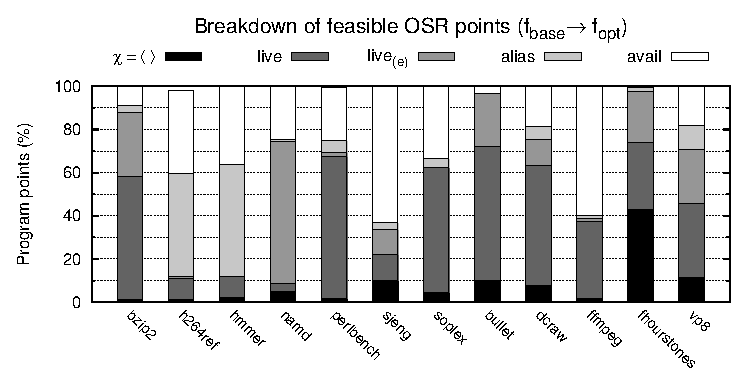
\includegraphics[width=0.8\textwidth]{figures/osr-BC-BtoO/osr-BC-BtoO.eps}
\caption{\protect\label{fig:osr-BC-BtoO} Fraction of program points that are OSR-feasible (from {\em base} to {\em opt}).

}
\end{center}
\end{figure}

We observe that the $live$ version of \reconstruct\ performs well on some benchmarks (e.g., \mytt{perlbench}, \mytt{bullet}, \mytt{dcraw}) and poorly on others (e.g., \mytt{h264ref}, \mytt{namd}). The enhancements introduced in the $live_{(e)}$ version are effective for some benchmarks (e.g., \mytt{namd}, \mytt{sjeng}), while aliasing information exploited in the $alias$ version increases the number of feasible OSR points for all benchmarks. For $9$ out of $12$ of them, it is possible in fact to build a compensation code using only live variables at the OSR source for more than $60\%$ of potential OSR points.

When in the $avail$ version \reconstruct\ is allowed to extend the liveness range of an ``available'' variable, the percentage of feasible OSR points grows to nearly $100\%$. We observed for \mytt{bullet} that a specific $\phi$-node needs to be reconstructed at nearly $20\%$ of feasible OSR points: this node takes as incoming values a number of $\phi$-nodes that in turn all yield the same value. While LLVM's built-in method for detecting trivially constant $\phi$-nodes does not cover this case, our recursive heuristic introduced in the $live_{(e)}$ version is able to identify the value and use it directly.

\begin{table}[!ht]
\begin{center}
\begin{small}
\begin{tabular}{ |c|c|c|c|c|c|c|c|c| }
\cline{2-9}
\multicolumn{1}{l|}{} & \multicolumn{2}{c|}{$|\chi|\leftarrow live_{(e)}$} & \multicolumn{2}{c|}{$|\chi|\leftarrow alias$} & \multicolumn{2}{c|}{$|\chi|\leftarrow avail$} & \multicolumn{2}{c|}{$|K_{avail}|$} \\
\hline
Benchmark & Avg & Max & Avg & Max & Avg & Max & Avg & Max \\
\hline
\hline
bzip2 & 4.29 & 14 & 4.3 & 14 & 4.73 & 13 & 3.6 & 8 \\
\hline
h264ref & 1.94 & 2 & 2.9 & 5 & 3.37 & 5 & 1.02 & 2 \\
\hline
hmmer & 3.3 & 5 & 16.11 & 23 & 16.63 & 24 & 4.02 & 7 \\
\hline
namd & 18.48 & 28 & 18.61 & 28 & 17.82 & 28 & 3.38 & 6 \\
\hline
perlbench & 46.29 & 57 & 46.12 & 57 & 45.82 & 57 & 1.24 & 12 \\
\hline
sjeng & 9.51 & 21 & 9.72 & 21 & 18.52 & 32 & 4.2 & 12 \\
\hline
soplex & 5.08 & 7 & 5.02 & 7 & 4.38 & 7 & 2.34 & 4 \\
\hline
bullet & 16.79 & 46 & 16.69 & 46 & 15.93 & 46 & 6.15 & 17 \\
\hline
dcraw & 7.72 & 15 & 7.6 & 15 & 7.32 & 15 & 1.97 & 7 \\
\hline
ffmpeg & 5.22 & 8 & 5.05 & 8 & 4.03 & 8 & 1.85 & 3 \\
\hline
fhourstones & 4.64 & 6 & 4.5 & 6 & 4.98 & 6 & 1.7 & 2 \\
\hline
vp8 & 9.6 & 16 & 10.51 & 16 & 10.13 & 17 & 2.35 & 6 \\
\hline
\hline
Mean & {\bf 11.07} & 18.75 & {\bf 12.26} & 20.50 & {\bf 12.81} & 21.50 & {\bf 2.82} & 7.17 \\
\hline
\end{tabular}
\end{small}
\end{center}
\caption{\label{tab:OSR-alC-prologue-BtoO} Average and peak size $|\chi|$ of the compensation code generated by the $live_{(e)}$, $alias$, and $avail$ versions of algorithm \reconstruct. $|K_{avail}|$ is the size of the set of variables that we should artificially keep alive in order to make program points represented by white bars in \myfigure\ref{fig:osr-BC-BtoO} feasible for an OSR from {\em base} to {\em opt}.}
\end{table}

In \mytable\ref{tab:OSR-alC-prologue-BtoO} we report the average and peak size of the compensation code $\chi$ generated by the $live_{(e)}$, $alias$, and $avail$ variants of \reconstruct\ across feasible OSR points. Figures for $live$ are not reported as they would not add much to the discussion. Note also that average values have been calculated for different sets of program points, although the set of a version includes the set of the previous version.

The assignment step of \reconstruct\ (line 9 in \myalgorithm\ref{alg:osr-reconstruct}, page \pageref{alg:osr-reconstruct}) generates an average number of instructions typically smaller than $20$, with the notable exception of \mytt{perlbench}. Observe that \mytt{perlbench}'s hottest function \mytt{S\_regmatch} is highly amenable to CSE: we found out that no less than $583$ out of its $667$ deleted instructions (thus about $10\%$ of the {\em base} function - see \mytable\ref{tab:OSR-alC-bench-IR}) are removed by this optimization, and we believe that local CSE would shrink the OSR entry block of the continuation function $f'$ as well. However, we would like to remark that the size of $\phi$ is unlikely to affect the performance of $f'$ for a hot method, as compensation code will be located at the beginning of the function and executed only once.

The last two columns of \mytable\ref{tab:OSR-alC-prologue-BtoO} report the average and peak number of variables that are not live at the source location, but for which the $avail$ version of \reconstruct\ would artificially extend liveness to support OSR at more program points (i.e., those represented by the white portions of the bars in \myfigure\ref{fig:osr-BC-BtoO}). We observe that the average number of values to spill on the stack is less than $3$ for $9$ out of $12$ benchmarks, with a maximum of $6.16$ for \mytt{bullet}. $avail$ by default will extend the liveness of an available value only if it is not possible to reconstruct it: this was implemented using a simple backtracking algorithm.

\subsection{OSR to Base Version}

\begin{figure}[!b]
\begin{center}
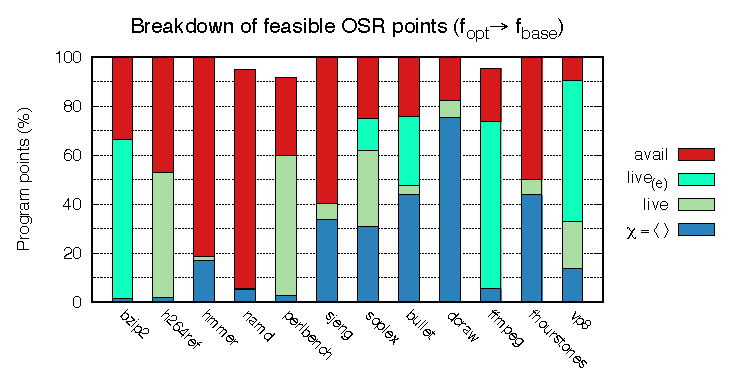
\includegraphics[width=0.8\textwidth]{figures/osr-BC-OtoB/osr-BC-OtoB.eps}
\caption{\protect\label{fig:osr-BC-OtoB} Fraction of program points that are OSR-feasible (from {\em opt} to {\em base}).


}
\end{center}
\end{figure}

\myfigure\ref{fig:osr-BC-OtoB} reports the fraction of OSR points eligible for {\em opt} to {\em base} deoptimization. We observe that the fraction of locations that can fire an OSR with an empty $\chi$ varies significantly from benchmark to benchmark, suggesting a dependence on the structure of the original program.

For $9$ out of $12$ benchmarks, compensation code can be built using only live variables for more than $50\%$ of potential OSR points.
%The assignment step of \reconstruct\ produces on average $2.3$ compensation instructions, with a peak of $5.74$ on \mytt{vp8}.
When the $avail$ version is used, the percentage of feasible OSR points is greater than $90\%$ on all benchmarks and nearly $100\%$ for $9$ out of $12$ of them.

Results for the $alias$ version of \reconstruct\ are not reported, as they do not improve those for $live_{(e)}$. Indeed, aliasing information is useful when a variable to set at destination is aliased by multiple variables at source, which we do not expect to happen in an optimized code.

\begin{table}[!ht]
\begin{center}
\begin{small}
\begin{tabular}{ |c|c|c|c|c|c|c| }
\cline{2-7}
\multicolumn{1}{l|}{} & \multicolumn{2}{c|}{$|\chi|\leftarrow live_{(e)}$} & \multicolumn{2}{c|}{$|\chi|\leftarrow avail$} & \multicolumn{2}{c|}{$|K_{avail}|$} \\
\hline
Benchmark & Avg & Max & Avg & Max & Avg & Max \\
\hline
\hline
bzip2 & 1.55 & 4 & 1.77 & 4 & 1.47 & 4 \\
\hline
h264ref & 4.46 & 9 & 2.82 & 9 & 1.45 & 7 \\
\hline
hmmer & 1 & 1 & 1 & 1 & 1.02 & 2 \\
\hline
namd & 1.5 & 2 & 5.93 & 15 & 4.74 & 18\\
\hline
perlbench & 4.09 & 12 & 4.22 & 12 & 1.37 & 11 \\
\hline
sjeng & 1.29 & 2 & 1.67 & 11 & 4.09 & 14 \\
\hline
soplex & 3.3 & 4 & 3.3 & 4 & 1.00 & 1 \\
\hline
bullet & 1 & 1 & 1.26 & 3 & 1.14 & 2 \\
\hline
dcraw & 1.68 & 2 & 3.84 & 6 & 4.06 & 8 \\
\hline
ffmpeg & 1.94 & 5 & 1.95 & 6 & 1.08 & 4 \\
\hline
fhourstones & 0 & 0 & 1.12 & 4 & 1.42 & 4 \\
\hline
vp8 & 5.74 & 13 & 5.51 & 13 & 1.18 & 5 \\
\hline
\hline
Mean & {\bf 2.30} & 4.58 & {\bf 2.87} & 7.33 & {\bf 2.00} & 6.67 \\
\hline
\end{tabular}
\end{small}
\end{center}
\caption{\label{tab:OSR-alC-prologue-OtoB} Average and peak size $|\chi|$ of the compensation code generated by the $live_{(e)}$ and $avail$ versions of algorithm \reconstruct. $|K_{avail}|$ is the size of the set of variables that we should artificially keep alive in order to make program points represented by white bars in \myfigure\ref{fig:osr-BC-OtoB} feasible for an OSR from {\em opt} to {\em base}.}
\end{table}

In \mytable\ref{tab:OSR-alC-prologue-OtoB} we report the average and peak size of the compensation code $\chi$ generated by the $live_{(e)}$ and $avail$ variants of \reconstruct\ across feasible OSR points, along with the average and peak number of available variables for which $avail$ artificially extends liveness to support OSR at program points represented by white bars in \myfigure\ref{fig:osr-BC-OtoB}. We observe that, compare to the {\em base}-to-{\em opt} case, the size of the compensation code is much smaller, suggesting that shorter portions of executions need to be reconstructed when OSR-ing to less optimized code.

Note that the $0$ values reported for \mytt{fhourstones} in the $live_{(e)}$ scenario do not imply that state compensation is not needed. In fact, the algorithm detected that each variable $v$ to assign at the OSR landing pad for which no live counterpart was available at the source location, could be initialized with the value of either a (non-live) function argument or some live variable when $v$ is a constant $\phi$-node. In LLVM IR assignments of the form \mytt{x:=y} are not allowed, since all uses of \mytt{x} can simply be replaced with uses of \mytt{y}: for this reason, a \mytt{RAUW(x,y)} operation is performed on the body of the continuation function $f'$, where \mytt{y} is a live value transferred as argument for $f'$, and no instruction is added to the OSR entry block of $f'$.
